\chapter{Classical Statistical Model}

\section{Probability versus statistical inference}

\textbf{Probability theory} begins with a completely specified model which we assume are correct and we compute the probabilities of certain events. 
For example, 
\begin{gather*}
    X_1,\ldots,X_n \overset{iid}{\sim} B(1,\theta)\\
    T = \sum_{i=1}^{n}X_i\sim B(n,\theta)\\
    P(T=t|\theta) = \left( \begin{array}{c} n \\ t \end{array} \right)\theta^t(1-\theta)^{n-t} \quad t=0,1,\ldots,n
\end{gather*}
with $n=20 \to P(T=10|\theta)$ is calculatable if we know $\theta$.
On the other hand, for \textbf{statistical inference}, we observe the realization of certain events,
and using that information we try to infer the probabilistic model that governs the corresponding random experiment. 
For example, $T=10\to$ observed outcome. I want to use this information to make inference about $\theta$.\\

\textbf{Statistical data} result from experiments conducted on a subset of a poopulation, the sample,
and we try to extend the conclusions obtained to the whole population.
\begin{center}
    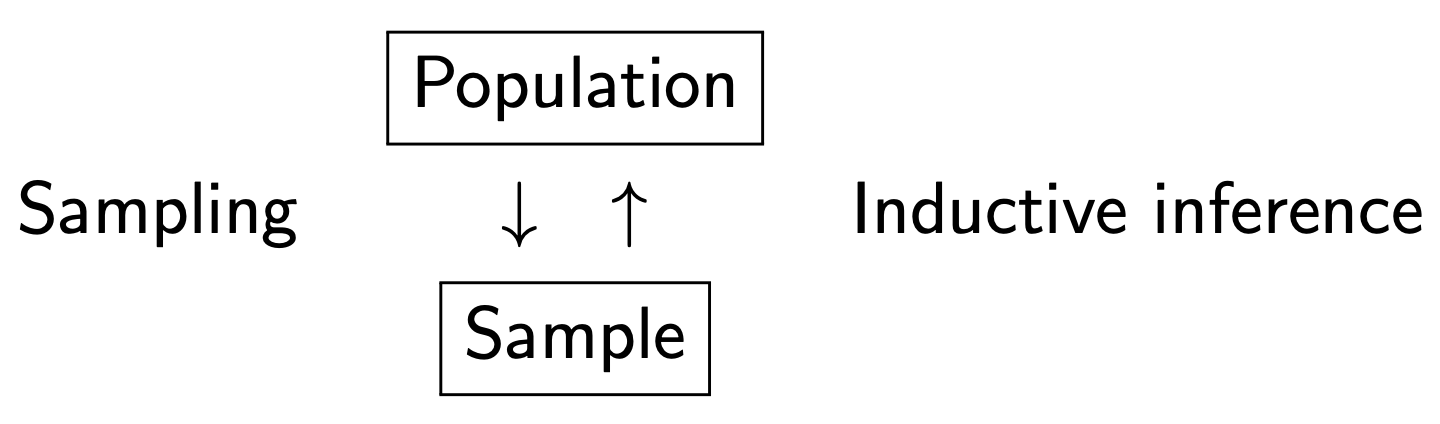
\includegraphics[scale=0.2]{Images/3.png}
\end{center}
\textbf{Inductive inference} means that there is uncertainty regarding the resulting inference.
If we are just drawing finite samples, then we cannot be certain the result is in fact representative of the entire population.
The opposite would be \textbf{deductive inference} where it is of mathematics. No questions about the validity of the inference.
If $A$ holds $\to B$ definitely holds.

\section{Model specification}

To formalize the process of statistical inference.
The characteristic of interest is modeled as a random variable $X$ with cumulative distribution function (cdf) $F$, the statistical model.
The model must be specified either through a \textbf{parametric model} where $F$ is a known up to a finite dimensional parameter, 
e.g. $X$ as normal with mean $\mu$ and variance $\sigma^2$, both unknown.
Or a \textbf{nonparametric model} where $F$ is specified in a nonparametric fashion, e.g. $F$ is an element f the set of all continuous and symmetric distribution.
Focusing on the parametric statistical model:
\begin{equation*}
    \mcF = \{F(\cdot|\theta):\underbrace{\theta}_{\text{parameter}}\in\underbrace{\Theta}_{\text{parameter space}}\}
\end{equation*}

\ex[]{Application : daily return of financial asset}{
    We can propose a normal $\to$
    $\mcF = \{N(\mu,\sigma^2):\mu\in\bbR,\sigma >0\}$
    or a gamma $\to$
    $\mcF = \{G(\alpha,\lambda):\alpha,\lambda >0\}$
}
\ex[]{Application : insurance policy}{
    If we are interested in the number of claims per year in an insurance policy, we can propose the Poisson
    $\to\mcF = \{Po(\lambda):\lambda >0\}$
}

The specificiation is important and results from many factors, namely based on the knowledge of the problem at hand, knowledge of previous studies, and knowledge of probability theory.
The consequence of model misspecification is always negative but is smaller for larger samples.

\subsection{Sampling}

\textbf{Random sampling} means that the observed data are one of many possible data sets we could have obtained in the same circumstances.
The set of $n$ observations, $(x_1,\ldots,x_n)$ which we have observed is a realization of an $n$-dimensional random variables $(X_1,\ldots,X_n)$.
\begin{equation*}
    \begin{split}
        (X_1,\ldots,X_n) & \qquad\text{Random sample}\\
        (x_1,\ldots,x_n) & \qquad\text{Observed sample}
    \end{split}
\end{equation*}
The \textbf{sample space} is a subset of $\bbR^n$ that contains the set of possible values for $x_1,\ldots,x_n$. We denoteit by $\mcX$.

\dfn[]{IID random sampling}{
    When the $n$ random variables that compose the random sample are
    \begin{itemize}
        \item mutually independent $\to x_i\ind x_j | \theta$
        \item identically distributed, with the same distribution as $X\to x_i\sim x_j | \theta$
    \end{itemize}
    we say that $(X_1,\ldots,X_n)$ constitutes an iid random sample of size $n$ obtained from the population $X$.
    In notation, $X_1,\ldots,X_n|\theta\overset{iid}{\sim}X$, $X$ follows the common distribution of all $x_i$'s, $x_i\sim X$.
}
If $\mcF = \{f(\cdot|\theta):\theta\in\Theta\}$ and $X_1,\ldots,X_n|\theta\overset{iid}{\sim} X$, then
\begin{equation*}
    \begin{split}
        F_{X_1,\ldots,X_n}(x_1,\ldots,x_n|\theta) & =\prod_{i=1}^{n}F_{X_i}(x_i|\theta)\qquad\text{by independence}\\
        & = \prod_{i=1}^{n}F(x_i|\theta)\qquad\text{since }X_i\sim X 
    \end{split}
\end{equation*}
and similarly for the probability density function
\begin{equation*}
    f(x_1,\ldots,x_n|\theta)=\prod_{i=1}^{n}f(x_i|\theta)
\end{equation*}
\begin{proof}
    \textbf{Poisson distribution}
    \begin{equation*}
        \begin{split}
            f(x_1,\ldots,x_n|\lambda) & = \prod_{i=1}^{n}f(x_i|\lambda)\\
            & = \prod_{i=1}^{n} e^{-\lambda}\frac{\lambda^{x_i}}{x_i!}\\
            & = P(x_1 = x_1,\ldots,x_n = x_n|\lambda)\\
            & = e^{-n\lambda}\frac{\lambda^{\sum_{i=1}^{n}x_i}}{\prod_{i=1}^{n}x_i!}\to\text{Annex 1}
        \end{split}
    \end{equation*}
    Annex 1: 
    \begin{itemize}
        \item $e^a e^b = e^{a+b}$
        \item $a^x a^y = a^{x+y}$
    \end{itemize}
\end{proof}

\section{Statistics}

\dfn[]{Statistic}{
    A statistic is any function of $(X_1,\ldots,X_n)$ that does not depend on unknown parameters.
}
\ex[]{Statistic}{
    In the context of a $N(\mu,\sigma^2)$, $\mu\in\bbR$ and $\sigma>0$ unknown.\\

    \textbf{Uni-dimensional} statistics include
    \begin{itemize}
        \item $T = \sum_{i=1}^{n}X_i$
        \item $\bar{X}=\frac{1}{n}T$
        \item $S^2 = \frac{1}{n}\sum_{i=1}^{n}(X_i-\bar{X})^2$
    \end{itemize}
    \textbf{Bi-dimensional} statistics include
    \begin{itemize}
        \item $(T, \sum_{i=1}^{n}X_i^2)$
        \item $(\bar{X},S^2)$
    \end{itemize}
}
\ex[]{Not statistic}{
    \begin{equation*}
        \sum_{i=1}^{n}(X_i-\mu)^2\qquad \frac{1}{\sigma^2}\sum_{i=1}^{n}X_i^2
    \end{equation*}
    are not statistics becuase they depend on unknown parameters. If $\sigma^2$ is known, then $\frac{1}{\sigma^2}\sum_{i=1}^{n}X_i^2$ is a statistic.
}

Statistics operate a data reduction and are summaries of the information contained in the random sample. 
Statistics are random variables, as usual, it is important to distinguish between the random variable and its observed value.
\begin{center}
    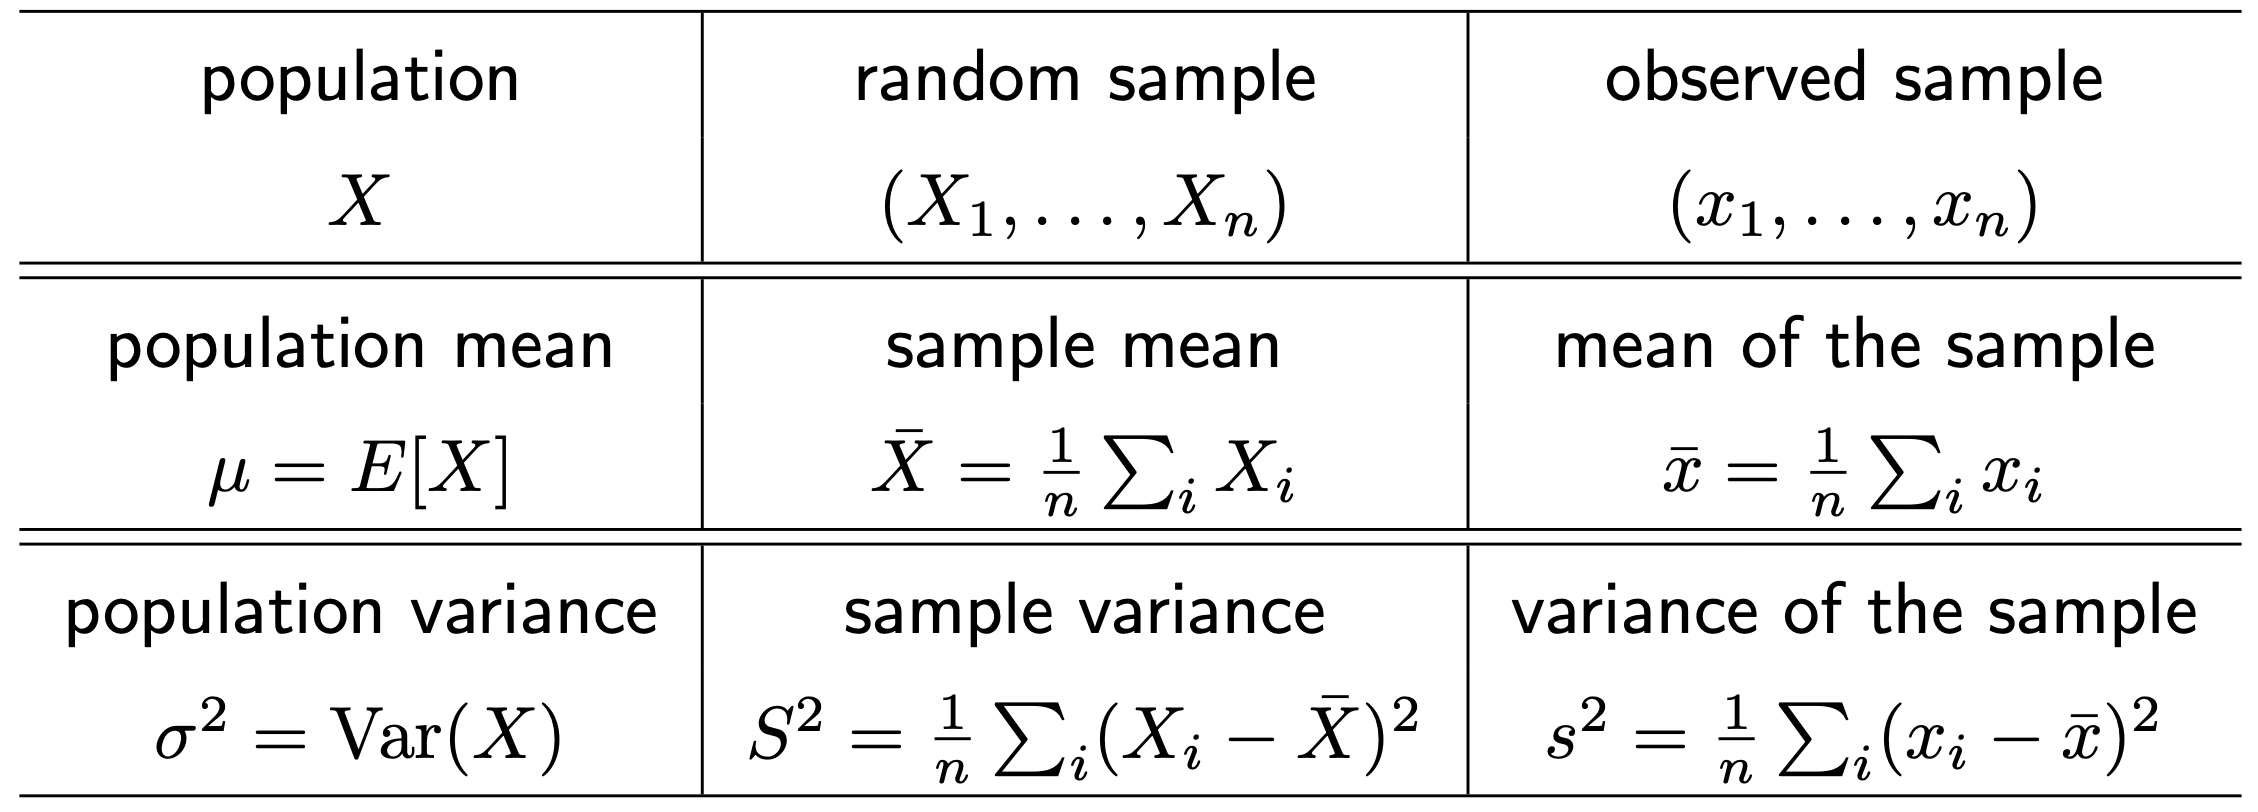
\includegraphics[scale=0.2]{Images/4.png}\\
    Probability vs. Statistics vs. Data exploration
\end{center}

\section{Sampling distribution}
The sampling distribution of a statistic corresponds to its probability distribution: as $(X_1,\ldots,X_n)$ varies according to its distribution,
what is the resulting probabilistic behavior of $T(X_1,\ldots,X_n)$. In classical inference, it is important to know the sampling distribution of statistics 
because that is necessary to evaluate the performance of statistical methodologies. The \textbf{objective} is to determine aspects of the sampling distribution
of a statistic $T$ knowing aspects of the probability distribution of the poopulation $X$.\\

There are different methods to obtain the sampling distribution of a statistic.
\begin{itemize}
    \item \textbf{Change of variable}: If $X$ is continuous,
        \begin{equation*}
            F_T(t|\theta) = P(T\leq t|\theta) = \int_{A(t)}\sum_{i=1}^{n}f(x_i|\theta)\, dx_1\ldots dx_n
        \end{equation*}
        where $A(t)=\{(x_1,\ldots,x_n)\in\bbR^n : T(x_1,\ldots,x_n)\leq t\}$. If $X$ is discrete, replace integrals with sums.
    \item Determining the \textbf{moment generating function} of $T$
    \item Using \textbf{well-known properties} of the distribution of $X$
    \item \textbf{Asymptotic approximations} to the sampling distribution of certain statistics (from CLT and related results)
    \item Using \textbf{simulations}
\end{itemize}
\ex[]{Change of variable}{
    Let $T = \sum_{i=1}^{n}X_i$
    \begin{itemize}
        \item If $(X_1,\ldots,X_n)$ is am iid random sample from a $Po(\lambda)$ population, since the sum of independent Poisson is still Poisson,
            we have $T\sim Po(n\lambda)$, hence $f_T(t|\lambda)= e^{-n\lambda}\frac{(n\lambda)^t}{t!},\, t\in N_0$.
        \item If $(X_1,\ldots,X_n)$ is an iid random sample from a $N(\mu,\sigma^2)$ population, then $T\sim N(n\mu, n\sigma^2)$.
        \item If $(X_1,\ldots,X_n)$ is an iid random sample from a $B(1,\theta)$ population, then $T\sim B(n,\theta)$.
    \end{itemize}
}
\ex[]{Monte Carlo simulation}{
    \begin{enumerate}
        \item Draw $N$ independent samples of size $n$ from the distribution of $X$
        \item For each of those samples, comptute the observed values of the statistic $T$
        \item The $N$ resulting numbers, $(t_1,\ldots,t_n)$ constitute a sample of size $N$ drawn from the sampling distribution of $T$
    \end{enumerate}
}

\subsection{Sample distribution of the sample moments}
\dfn[]{Sample moments}{
    Let $(X_1,\ldots,X_n)$ be an iid random sample of size $n$ from a population $X$. 
    For $k\in\bbN$ we define the $k$th raw sample moment as
    \begin{equation*}
        M'_k=\frac{1}{n}\sum_{i=1}^{n}x_i^k
    \end{equation*}
    and the $k$th central sample moment by
    \begin{equation*}
        M_k = \frac{1}{n}\sum_{i=1}^{n}(X_i-\bar{X})^k
    \end{equation*}
}
$\begin{cases*}
    \mu'_k = E[x^k] \to k\text{th raw moment}\\
    M'_k = \frac{1}{n}\sum x_i^k\to k\text{th sample raw moment}
\end{cases*}$ 
$\begin{cases*}
    \mu_k = E[(x-\mu)^k] \to k\text{th central moment}\\
    M_k = \frac{1}{n}\sum (x_i-\bar{x})^k\to k\text{th central sample moment}
\end{cases*}$\\
We want to observe how they behave in relation to each other.\\

Once again, it is important to distinguish the \textbf{sample moments}, $M'_k$ and $M_k$,
from the \textbf{population momnets}, $\mu'_k = E[X^k]$ and $\mu_k = E[(X-E[X])^k]$,
and the \textbf{observed sample moments}, $m'_k = \frac{1}{n}\sum_{i=1}^{n}x_i^k$ and $m_k = \frac{1}{n}\sum_{i=1}^{n}(x_i-\bar{x})^k$.

\nt{
    \textbf{Important special cases: }$\bar{X} = M'_1$ and $S^2 = M_2$, the sample mean and the sample variance.
}

\thm[]{Properties of the sample mean}{
    If all the moments exist, then
    \begin{align*}
        E[\bar{X}] & = E[X] = \mu\\
        Var(\bar{X}) & = \frac{Var(X)}{n} = \frac{\sigma^2}{n}\\
        \mu_3 & = \frac{\mu_3}{n^2}\\
        \mu_4 & = \frac{3\mu_2^2}{n^2} + \frac{\mu_4-3\mu_2^2}{n^3}
    \end{align*}
}
\begin{proof}
    \textbf{$E[\bar{X}]$}
    \begin{equation*}
        E[\bar{X}] = \frac{1}{n}\sum_{i=1}^{n}E[x_i] = \frac{1}{n}n\mu = \mu
    \end{equation*}
\end{proof}
\begin{proof}
    $Var(\bar{X})$
    \begin{align*}
        Var(\bar{X}) & = E[(\bar{X}-\mu)^2]\\
        & = E[(\frac{1}{n}\sum x_i-\mu)^2]\\
        & = E[\frac{1}{n^2}(\sum(x_i-\mu))^2]\\
        & = \frac{1}{n^2}E[\overbrace{(\sum \underbrace{a_i}_{= x_i-\mu})^2}^{\text{Annex 1}}]\\
        & = \otimes
    \end{align*}
    Annex 1: $(\sum a_i)^2 = (\sum_i a_i)(\sum_j a_j) = \sum_i \sum_j a_ia_j = \sum_i a_i^2 + \sum_i \sum_{i\neq j}a_ia_j \qquad\square$
    \begin{align*}
        \otimes & = \frac{1}{n^2}[E[\sum_i a_i^2] + E[\sum_i \sum_{i\neq j}a_ia_j]]\\
        & = \frac{1}{n^2}[\sum_i \underbrace{E[a_i^2]}_{E[(X-\mu)^2] = Var(X) = \sigma^2} + \sum_i \sum_{i\neq j}\underbrace{E[a_ia_j]}_{\text{Cov}(a_i,a_j) = 0\to\text{ Annex 2}}]\\
        & = \frac{1}{n^2}(n\sigma^2 + 0)\\
        & = \frac{\sigma^2}{n}
    \end{align*}
    Annex 2: Since $a_i\ind a_j$, expectation of the product is the product of the expectation for independent variables.
    This implies that $E[(x_i-\mu)(x_j-\mu)] = E[(x_i-\mu)]E[(x_j-\mu)] = 0\times 0 = 0$
\end{proof}
By the \textbf{Weak Law of Large Numbers}, $\bar{X}\overset{P}{\to}\mu$. The distribution is more and more concentrated around $\mu$ as $n$ increases. 
The distribution of $\bar{X}$ is centered around $\mu$ and $\lim_{n\to+\infty}Var(\bar{X}) = 0$.
\begin{proof}
    Asymmetry $\mu_3$
    \begin{equation*}
        \mu_3(\bar{X}) = E[(\bar{X}-\mu)^3] = \frac{1}{n^3}E[\underbrace{(\sum a_i)^3}_{\text{Annex 1}}] = \otimes
    \end{equation*}
    Annex 1: 
    \begin{align*}
        (\sum a_i)^3 & = (\sum_i a_i)(\sum_j a_j)(\sum_k a_k) = \sum_i\sum_j\sum_k a_ia_ja_k\\
        & = (\sum a_i)^2(\sum_k a_k) = (\sum_i a_i^2 + \sum_i\sum_{i\neq j}a_ia_j)(\sum_k a_k)\\
        & = \sum_i\sum_k a_i^2 a_k + \sum_i\sum_{i\neq j}\sum_k a_ia_ja_k\\
        & = \sum_i a_i^3 + \underbrace{\sum_i\sum_{k\neq i}a_i^2 a_k}_{E[\cdot]=0} + \underbrace{\sum_i\sum_{j\neq i}\sum_{k\neq i}a_ia_ja_k}_{E[\cdot]=0}
        + \underbrace{\sum_i\sum_{j\neq i}a_i^2 a_j}_{E[\cdot]=0}\qquad\square
    \end{align*}
    \begin{equation*}
        \otimes = \frac{1}{n^3}\sum_{i=1}^{n}E[(x_i-\mu)^3] = \frac{1}{n^3}n\mu_3 = \frac{\mu_3}{n^2}\xrightarrow{n\to\infty} 0
    \end{equation*}
\end{proof}
As $n$ goes to infinity, the distribution becomes symmetric. This evidence is compatible with the \textbf{Central Limit Theorem}.
The related concept to asymmetry is \textbf{skewness}, $\gamma_1 = \frac{\mu_3}{\sigma^3}$. 
$\sigma^3$ is used to make $\gamma_1$ dimensionless, as in independent of the unit measurement of the $x$.\\

The commonly used concept related to $\mu_4$ is \textbf{kurtosis} which is often denoted as $\gamma_2 = \frac{\mu_4}{\sigma^4}$. 
It is the indication of heavy tails. If $\gamma_2 > 3$, the distribution has a heavier tail than Gaussian.
The excess kurtosis can also be used which is just $\gamma_2 - 3$, indicating heavier tail than Gaussian if bigger than 0.
\begin{proof}
    Kurtosis $\gamma_2$
    \begin{align*}
        \gamma_2(\bar{X}) & = \frac{\mu_4(\bar{X})}{\underbrace{\sigma_{(\bar{X})}^4}_{\text{s.d. to the power of 4}}} = \frac{\frac{3\mu_2^2}{n^2}+\frac{\mu_4-3\mu_2^2}{n^3}}{(\sqrt{\frac{\sigma^2}{n}})}\\
        & = \frac{\frac{3\mu_2^2}{n^2}+\frac{\mu_4-3\mu_2^2}{n^3}}{(\frac{(\sigma^2)^2}{n^2})} \overset{\mu_2 = \sigma^2}{=} \frac{\frac{3\mu_2^2}{n^2}+\frac{\mu_4-3\mu_2^2}{n^3}}{(\frac{(\mu_2)^2}{n^2})}\\
        & = 3 + \frac{1}{n}\underbrace{\frac{\mu_4-3\mu_2^2}{\mu_2^2}}_{\text{A}}\xrightarrow{n\to\infty} 3
    \end{align*}
    A: $\frac{\mu_4}{\mu_2^2}-\frac{3\mu_2^2}{\mu_2^2} = \frac{\mu_4}{\sigma^4}-3 \to \gamma_2 - 3 \Rightarrow$ excess kurtosis.\\
\end{proof}

\thm[]{Properties of the sample variance}{
    If all the moments exist,
    \begin{align*}
        E[S^2] & = \frac{n-1}{n}\sigma^2\\
        Var(S^2) & = \frac{\mu_4-\mu_2^2}{n}-2\frac{\mu_4-2\mu_2^2}{n^2}+\frac{\mu_4-3\mu_2^2}{n^3} \xrightarrow{n\to\infty} 0\text{ , roughtly centered around }S^2
    \end{align*}
}
Since $E[S^2] = \frac{n-1}{n}\sigma^2 < \sigma^2$, always strictly smaller than the variance, we define the \textbf{bias-corrected sample variance}
\begin{equation*}
    S'^2 = \frac{1}{n-1}\sum_{i=1}^{n}(X_i-\bar{X})^2 = \frac{n}{n-1}S^2
\end{equation*}
Notice that $M'_k = \frac{1}{n}\sum X_i^k$ which is the average of iid r.v. but $M_k = \frac{1}{n}\sum (X_i-\bar{X})^k$.
We cannot use LLN or CLT to study $M_k$ becuase $(X_i-\bar{X})$ and $(X_j-\bar{X})$ for $i\neq j$ are not iid as $\bar{X}$ depends on both $X_i$ and $X_j$.

\thm[]{Properties of the bias-corrected sample variance}{
    If all the moments exist,
    \begin{align*}
        E[S'^2] & = \sigma^2\\
        Var(S'^2) & = \frac{1}{n}(\mu_4 - \frac{n-3}{n-1}\mu_2^2)
    \end{align*}
}
\begin{proof}
    $E[S'^2]$
    \begin{align*}
        S'^2 & = \frac{nS^2}{n-1}\\
        E[S'^2] & = \frac{n}{n-1}E[S^2] = \frac{n}{n-1}\frac{n-1}{n}\sigma^2 = \sigma^2
    \end{align*}
\end{proof}

\thm[]{Properties of central sample moments}{
    If all the moments exist,
    \begin{align*}
        E[M_k] & = \mu_k + \mcO(\frac{1}{n})\\
        Var(S'^2) & = \frac{c}{n} + \mcO(\frac{1}{n^2})
    \end{align*}
    where $c$ is a constant which involves central population moments of order $\leq 2k$.
}
The central sample moments have similar behavior as $S^2$.
\begin{align*}
    a_n & = \mcO(b_n) \Leftrightarrow \frac{a_n}{b_n} \text{ is limited}\\
    a_n & = \mcO(\frac{1}{n}) \Leftrightarrow \frac{a_n}{\frac{1}{n}} \text{ is limited} = na_n\\
    a_n & = \underbrace{\frac{1}{n}}_{\to 0}\underbrace{na_n}_{\text{limited}} \to 0\\
    & \Rightarrow \mcO(\frac{1}{n}) \text{ sequence goes to 0 roughtly at the rate of }\frac{1}{n}
\end{align*}

\thm[]{Asymptotic distribution of $\bar{X}$}{
    As long as $Var(X)$ is finite, we have as a direct consequence of the \textbf{Central limit theorem} that
    \begin{equation*}
        \frac{\bar{X}-\mu}{\frac{\sigma}{\sqrt{n}}} = \sqrt{n}\frac{\bar{X}-\mu}{\sigma}\xrightarrow{d}N(0,1)
    \end{equation*}
}
This result is typically used in the form
\begin{equation*}
    P(\bar{X}\leq x)\approx \Phi\left(\sqrt{n}\frac{x-\mu}{\sigma}\right)
\end{equation*}
that is, $\bar{X}\overset{a}{\sim}N(\mu,\frac{\sigma^2}{n})$.\\

In general, unimodality and symmetry have a positive impact on the speed of convergence. If the distribution is already behaving like normal, the rate of convergence would be faster.

\subsection{Order statistics}
\dfn[]{Order statistics}{
    Let $(X_1,\ldots,X_n)$ be an iid random sample. The $i$th order statistic is denoted by $X_{(i)}$ and satisfies
    \begin{equation*}
        \underbrace{X_{(1)} \leq X_{(2)} \leq \ldots \leq X_{(n)}}_{\text{not iid}}
    \end{equation*}
}
Order statistics are not iid because if we know $X_{(n)}$ is 10, then $X_{(1)}$ cannot be larger than 10. 
For notation purposes, $(Y_1, \ldots,Y_n) \equiv (X_{(1)},\ldots,X_{(n)})$.\\

The order statistics have a joint pdf given by
\begin{equation*}
    g(y_1,y_2,\ldots,y_n) = n!\prod_{i=1}^{n}f(y_i)\qquad \text{if } y_1 < y2 < \ldots < y_n
\end{equation*}
If $u>v$, the joint pdf of $(Y_u,Y_v)$ is
\begin{equation*}
    g_{u,v}(y,z) = \frac{n!}{(u-1)!(v-u-1)!(n-v)!}\times[F(y)]^{u-1}[F(z)-F(y)]^{v-u-1}[1-F(z)]^{n-v}f(y)f(z)\quad \text{if }y<z
\end{equation*}
The cdf of $Y_v$ is
\begin{equation*}
    g_v(y) = \frac{n!}{(v-1)!(n-v)!}[F(y)]^{v-1}[1-F(y)]^{n-v}f(y) = G'_v(y)
\end{equation*}
and the pdf of $Y_v$ is
\begin{equation*}
    G_v(y) = \sum_{j=v}^{n}\left(\begin{array}{c}
    n\\j\end{array}\right)[F(y)]^j[1-F(y)]^{n-j} = P(Y_v\leq y)
\end{equation*}

\begin{proof}
    The joint distribution of $G_{u,v}(y,z)$ follows a \textbf{multinomial distribution} with the following characteristics:
    \begin{itemize}
        \item $n$ objects
        \item $k$ categories
        \item The probability that each object belongs to category $i$ is $p_i$, $i=1,\ldots,k$ independently
        \item $w_i$ is the number of objects among the $n$ that belongs to class $i$, $i=1,\ldots,k$
    \end{itemize}
    \begin{align*}
        G_{u,v}(y,z) & = P(Y_u\leq y, Y_v\leq z)\\
        g_{u,v}(y,z) & = \frac{\partial^2 G(y,z)}{\partial y\partial z} = \lim_{\delta_1\to0^+,\delta_2\to0^+}P(y<y_u\leq y+\delta_1, z<y_v\leq z+\delta_2)
    \end{align*}
    This is a multinomial with 5 classes:
    \begin{equation*}
        \begin{cases*}
            P_1 = F(y)\\
            P_2 = P(y<x\leq y+\delta_1) = F(y+\delta_1)-F(y)\\
            P_3 = F(z)-F(y+\delta_1)\\
            P_4 = P(z<x\leq z+\delta_2) = F(z+\delta_2)-F(z)\\
            P_5 = 1-F(z+\delta_2)
        \end{cases*}
    \end{equation*}
    with \begin{equation*}
        \begin{cases*}
            w_1 = u-1\\
            w_2 = 1\\
            w_3 = v-u-1\to\text{Annex 1}\\
            w_4 = 1\\
            w_5 = n-v
        \end{cases*}
    \end{equation*}
    Annex 1: $n = u-1+1+1+n-v+w_3\Leftrightarrow n=u+1+n-v+w_3\Leftrightarrow w_3=n-u-1-n+v=v-u-1$\\
    where \begin{equation*}
        P(y<Y_u\leq y+\delta_1, z<Y_v\leq z+\delta_2) = \frac{n!}{(u-1)!1!(v-u-1)!1!(n-v)!}P_1^{u-1}P_2^1 P_3^{v-u-1} P_4^1 P_5^{n-v}
    \end{equation*}
    thus,
    \begin{align*}
        g_{u,v}(y,z) & = \lim_{\delta_1\to0^+,\delta_2\to0^+}\frac{n!}{(u-1)!(v-u-1)!(n-v)!}[F(y)]^{u-1}[F(y+\delta_1)-F(y)]\\
        & \times [F(z)-F(y+\delta_1)]^{v-u-1}[F(z+\delta_2)-F(z)][1-F(z+\delta_2)]^{n-v}\\
        & = \frac{n!}{(u-1)!(v-u-1)!(n-v)!}[F(y)]^{u-1}[F(z)-F(y)]^{v-u-1}[1-F(z)]^{n-v}\\
        & \times \underbrace{\lim_{\delta_1\to0^+}\frac{F(y+\delta_1)-F(y)}{\delta_1}}_{f(y)}\underbrace{\lim_{\delta_2\to0^+}\frac{F(z+\delta_2)-F(z)}{\delta_2}}_{f(z)}\\
        & = \frac{n!}{(u-1)!(v-u-1)!(n-v)!}[F(y)]^{u-1}[F(z)-F(y)]^{v-u-1}[1-F(z)]^{n-v}f(y)f(z)
    \end{align*}
\end{proof}
\begin{proof}
    The cdf of $Y_v$
    \begin{align*}
        G_v(y) & = P(Y_v\leq y) = P(\text{at least }v\text{ of the }X_i\text{'s are }\leq y)\\
        & = \underbrace{\sum_{j=v}^{n}P(\text{exactly }j\text{ of the }X_i\text{'s are }\leq y)}_{N_y=\#\{i:x_i\leq y\}}\\
        & = \sum_{j=v}^{n}\left(\begin{array}{c}
        n\\j\end{array}\right)[F(y)]^j[1-F(y)]^{n-j}\quad \text{since }N_y\sim B(n,F(y))
    \end{align*}
    The pdf is just the derivative of the cdf, thus
    \begin{align*}
        g_v(y) & = G'_v(y) = \sum_{j=v}^{n}\left(\begin{array}{c}
        n\\j\end{array}\right)\left[j[F(y)]^{j-1}f(y)[1-F(y)]^{n-j} - [F(y)]^j(n-j)[1-F(y)]^{n-j-1}(-f(y))\right]\\
        & = f(y)\sum_{j=v}^{n}\left(\begin{array}{c}
        n\\j\end{array}\right)[F(y)]^{j-1}[1-F(y)]^{n-j}[j + n - j - nj]\\
        & = f(y)\sum_{j=v}^{n}\left(\begin{array}{c}
        n\\j\end{array}\right)[F(y)]^{j-1}[1-F(y)]^{n-j}[n - nj + j]\\
        & = f(y)\sum_{j=v}^{n}\left(\begin{array}{c}
        n\\j\end{array}\right)[F(y)]^{j-1}[1-F(y)]^{n-j}[n(1 - j) + j]\\
        & = f(y)\sum_{j=v}^{n}\left(\begin{array}{c}
        n\\j\end{array}\right)[F(y)]^{j-1}[1-F(y)]^{n-j}[n - nj + j]\\
        & = \frac{n!}{(v-1)!(n-v)!}[F(y)]^{v-1}[1-F(y)]^{n-v} f(y)
    \end{align*}
\end{proof}

\thm[]{Important special cases : the maximum and the minimum}{
    The pdf and the cdf of the minimum and the maximum are
    \begin{align*}
        G_1(y) & = 1- [1-F(y)]^n & g_1(y) & = n\, f(y)[1-F(y)]^{n-1}\\
        G_n(y) & = [F(y)]^n & g_n(y) & = n\, f(y)[F(y)]^{n-1}\\
    \end{align*}
    with the joint cdf of
    \begin{equation*}
        g_{1,n}(y,z)=n(n-1)[F(z)-F(y)]^{n-2}f(y)f(z)\qquad y<z
    \end{equation*}
}
\begin{proof}
    $G_n(y)$
    \begin{align*}
        G_n(y) & = P(Y_n\leq y) = P(X_{(n)}\leq y)\\
        & = P(X_{(1)}\leq y,\ldots, X_{(n)}\leq y) \to \text{Annex 1}\\
        & = P(X_{(1)}\leq y)\,P(X_{(2)}\leq y)\cdots P(X_{(n)}\leq y)\quad \text{because }x_i\ind x_j, i\neq j\\
        & = [F(y)]^n\quad \text{because iid}
    \end{align*}

    Annex 1: If $X_{(n)}\leq y\Leftrightarrow X_{(1)}\leq y,\ldots, X_{(n)}\leq y$\\

    $g_n(y) = G'_n(y)$ if continuous\\
\end{proof}
\begin{proof}
    $G_1(y)$\\

    The idea is that
    \begin{equation*}
        X_{(1)}\leq y \Leftrightarrow \exists_i X_i \leq y
    \end{equation*}
    Thus we can write
    \begin{align*}
        G_1(y) & = P(X_{(1)}\leq y) = P(\exists_i X_i\leq y)\\
        & = P(\overline{\forall_i X_i>y}) = 1-P(\forall X_i>y)\\
        & = 1 - P(X_{(1)}>y, \ldots, X_{(n)}>y) = 1 - P(X_{(1)}>y)\cdots P(X_{(n)}>y) \quad \text{because }x_i\ind x_j, i\neq j\\
        & = 1 - [1-F(y)]^n \quad \text{because iid}
    \end{align*}
\end{proof}
\begin{proof}
    $g_{1,n}(y,z)$
    \begin{align*}
        G_n(y) & = G_{1,n}(x,y) + P(x<X_i\leq y, \forall i)\\
        & = G_{1,n}(x,y) + \underbrace{[F[(y) - F(x)]^n}_{P(a<X\leq b) = F(b)-F(a)}\quad \text{justified through \textbf{total probability theorm}}\\
        \Leftrightarrow [F(y)]^n & = G_{1,n}(x,y) + [F(y)-F(x)]^n\\
        \Leftrightarrow G_{1,n}(x,y) & = [F(y)]^n - [F(y)-F(x)]^n \, ,x<y
    \end{align*}
    The cumulative distribution function is just the derivative relative to both variables, so
    \begin{align*}
        g_{1,n}(x,y) & = \frac{\partial^2}{\partial y\partial x}G_{1,n}(x,y)\\
        & = \frac{\partial}{\partial y}[0-n(-f(x))[F(y)-F(x)]^{n-1}]\\
        & = nf(x)(n-1)f(y)[F(y)-F(x)]^{n-2}\, ,n>2
    \end{align*}
\end{proof}
\ex[]{Pareto}{
    Pareto distribution is one of the fat tail distributions.
    \begin{equation*}
        f(x) \propto x^{-(\theta+1)}\, ,x>c \Leftrightarrow f(x) = bx^{-(\theta+1)}
    \end{equation*}
    To find $b$, we impose that the integral of the pdf is equal to 1.
    \begin{align*}
        \int_{c}^{+\infty}bx^{-(\theta+1)}\,dx & = 1\\
        b\left[-\frac{1}{\theta}x^{-\theta}\right]_{c}^{+\infty} & = 1\\
        b\left(0-\frac{c^{-\theta}}{-\theta}\right) & = 1\\
        b\frac{c^{-\theta}}{\theta} & = 1\\
        b & = \theta c^{\theta}
    \end{align*}
    Polynomial decays slower than exponential decays. This means that the tails are heavier.
    \begin{align*}
        F(x) & = P(X\leq x) = \int_{c}^{x} f(u) \, du\\
        & = \int_{c}^{x} \theta c^{\theta} u^{-(\theta+1)}\, du\\
        & = \theta c^{\theta}\left[-\frac{u^{-\theta}}{\theta}\right]_{c}^{x}\\
        & = \theta c^{\theta}\left(\frac{x^{-\theta}-c^{-\theta}}{-\theta}\right)\\
        & = c^{\theta}(c^{-\theta}-x^{-\theta})\\
        & = 1 - \left(\frac{c}{x}\right)^{\theta}\\
        & = 1 - c^\theta x^{-\theta}\, ,x>c
    \end{align*}
    Now showing the distribution of the minimum order statistic.
    \begin{align*}
        g_1(y) & = n f(y)[1-F(y)]^{n-1}\\
        & = n \theta c^{\theta} y^{-(\theta+1)}\left[c^{\theta} y^{-\theta}\right]^{n-1}\\
        & = n \theta c^{\theta} y^{-(\theta+1)} c^{\theta(n-1)} y^{-\theta(n-1)}\\
        & = n \theta c^{\theta n} y^{-(\theta n + 1)}\, ,y>c
    \end{align*}
    This has the same structure as a Pareto distribution with parameter $\theta n$.
    Thus, the minimum of a sample of size $n$ from a Pareto($\theta$) distribution is still a Pareto distribution with parameter $\theta n$.
    \begin{equation*}
        X_{(1)} \sim Pa(c, \theta n)
    \end{equation*}
    However, the maximum does not have a simple form.
    \begin{equation*}
        g_n(y) = n \theta c^{\theta} y^{-(\theta+1)}\left[1 - c^{\theta} y^{-\theta}\right]^{n-1}\, ,y>c
    \end{equation*}
    The maximum does not belong to the Pareto family.
}
\ex[]{Exponential}{
    Let $(X_1,\ldots,X_n)$ be an iid random sample from an $Exp(\lambda)$ population.
    The pdf and cdf of the exponential distribution are
    \begin{equation*}
        f(x) = \lambda e^{-\lambda x}\, ,x>0\quad\quad F(x) = 1 - e^{-\lambda x}\, ,x>0
    \end{equation*}
    The pdf of the minimum order statistic is
    \begin{align*}
        g_1(y) & = n f(y)[1-F(y)]^{n-1}\\
        & = n \lambda e^{-\lambda y}\left[e^{-\lambda y}\right]^{n-1}\\
        & = n \lambda e^{-\lambda y} e^{-\lambda ny+\lambda y}\\
        & = n \lambda e^{-\lambda n y}\, ,y>0
    \end{align*}
    This has the same structure as an exponential distribution with parameter $\lambda n$.
    Thus, the minimum of a sample of size $n$ from an $Exp(\lambda)$ distribution is still an exponential distribution with parameter $\lambda n$.
    \begin{equation*}
        X_{(1)} \sim Exp(\lambda n)
    \end{equation*}
    Also notice that
    \begin{equation*}
        E[x] = \frac{1}{\lambda} \Rightarrow E[X_{(1)}] = \frac{1}{\lambda n} < \frac{1}{\lambda}
    \end{equation*}
    This makes sense as it is often used to model duration.\\
    The pdf of the maximum order statistic is
    \begin{align*}
        g_n(y) & = n f(y)[F(y)]^{n-1}\\
        & = n \lambda e^{-\lambda y}\left[1 - e^{-\lambda y}\right]^{n-1}\, ,y>0
    \end{align*}
    The maximum does not belong to the exponential family.
}

\dfn[]{Sample quantile}{
    Let $p\in(0,1)$ and $k=np$. Then the sample quantile of order $p$ is $Z_p$ such that
    \begin{equation*}
        Z_p = \begin{cases*}
            \frac{Y_k+Y_{k+1}}{2} & if $k$ is an integer\\
            Y_{(\lceil k \rceil)} & if $k$ is not an integer
        \end{cases*}
    \end{equation*}
    where $\lceil k \rceil$ is the integer part of $k$.
}
\thm[]{Asymptotic distribution of the sample quantile of order $p$}{
    Let $Z_p$ be the sample quantile of order $p$ of an iid random sample of size $n$, obtained from a continuous population with density $f$. 
    Denoted by $\xi_p$ the population quantile of order $p$.
    If $f$ is continuous and positive at $\xi_p$, then
    \begin{equation*}
        \sqrt{n}\, f(\xi_p) \frac{Z_p - \xi_p}{\sqrt{p(1-p)}}\xrightarrow{d} N\left(0, 1\right)
    \end{equation*}
}
\begin{equation*}
    \xi_p : P(X\leq \xi_p) \geq p \quad\text{and}\quad P(X\geq\xi_p)\geq 1-p
\end{equation*}
If $X$ is continous, $F(\xi_p) = p$. It is actually quite difficult to prove the relationship between the population quantle $\xi_p$ and the sample quantile $Z_p$.
\ex[]{Normal}{
    If $X\sim N(\mu,\sigma^2)$, then $\xi_{\frac{1}{2}} = \mu$. Then $f(\xi_{\frac{1}{2}}) = (2\pi\sigma^2)^{-\frac{1}{2}}$. Hence,
    \begin{equation*}
        \sqrt{n}\frac{Z_{\frac{1}{2}} - \mu}{\sigma}\xrightarrow{d} N(0, \frac{\pi}{2}) \Leftrightarrow \sqrt{\frac{2n}{\pi\sigma^2}}(Z_{\frac{1}{2}}-\mu)\xrightarrow{d}N(0,1)
    \end{equation*}
}

\thm[]{Fisher-Tippett-Gnedenko Theorem}{
    If $\exists a_n, b_n\, ,b_n>0$ then
    \begin{equation*}
        \lim_{n\to\infty} P\left(\frac{X_{(n)} - a_n}{b_n} \leq x\right) = F(x)
    \end{equation*}
    and $F$ is the cdf of a non-degenerate r.v., then $F$ belongs to one of the following three families:
    \begin{itemize}
        \item \textbf{Gumbel} : $F(x) = e^{-e^{-(x-\mu)/\beta}}\, ,x\in\mathbb{R}$, with $\mu\in\mathbb{R}$ and $\beta>0$
        \item \textbf{Fréchet} : $F(x) = 0\, ,x\leq \mu$ and $F(x) = e^{-((x-\mu)/\beta)^{-\alpha}}\, ,x>\mu$ with $\mu\in\mathbb{R}$, $\beta>0$ and $\alpha>0$
        \item \textbf{Weibull} : $F(x) = e^{-((\mu - x)/\beta)^{\alpha}}\, ,x<\mu$ and $F(x) = 1\, ,x\geq \mu$ with $\mu\in\mathbb{R}$, $\beta>0$ and $\alpha>0$
    \end{itemize}
    One of the three extreme value distributions.
}

\subsection{A few sampling distributions}

\subsubsection{Normal population}
Let $(X_1,\ldots,X_n)$ be an iid random sample from a $N(\mu,\sigma^2)$ distribution.
\begin{itemize}
    \item Distribution of the sample mean $\bar{X}$\\
    
        $\bar{X}$ is a linear combination of independent normals, hence it follows a normal distribution. We know that $E[\bar{X}] = \mu$ and $Var(\bar{X}) = \frac{\sigma^2}{n}$. Thus,
        \begin{equation*}
            \bar{X} \sim N\left(\mu, \frac{\sigma^2}{n}\right)\quad \text{or}\quad \sqrt{n}\frac{\bar{X}-\mu}{\sigma} \sim N(0,1)
        \end{equation*}
        Unlike the CLT which is approximately $N(0,1)$, this is exact.
    \item Distribution of the bias-corrected sample variance $S'^2$\\
    
        Because $\frac{X_i - \mu}{\sigma}\sim N(0,1)$, we have $\left(\frac{X_i-\mu}{\sigma}\right)^2\sim \chi^2_1$. 
        Thus, $\sum_{i=1}^{n}\left(\frac{X_i-\mu}{\sigma}\right)^2\sim \chi^2_n$.\\

        Also $\sum_{i=1}^{n}(X_i - \mu)^2 = \sum_{i=1}^{n}[(X_i - \bar{X}) + (\bar{X} - \mu)]^2 = \sum_{i=1}^{n}(X_i - \bar{X})^2 + n(\bar{X} - \mu)^2$.
        Hence, 
        \begin{equation*}
            \sum_{i=1}^{n}(X_i - \mu)^2 = (n-1)\frac{S'^2}{\sigma^2} + n\frac{(\bar{X} - \mu)^2}{\sigma^2}
        \end{equation*}
        Since $\bar{X}\sim N(\mu,\frac{\sigma^2}{n})$, we have $n\frac{(\bar{X} - \mu)^2}{\sigma^2}\sim \chi^2_1$.
        Also, $\bar{X}$ and $S'^2$ are independent in the context of the normal distribution.
        Thus, \begin{equation*}
            (n-1)\frac{S'^2}{\sigma^2} = \sum_{i=1}^{n}(X_i - \mu)^2 - n\frac{(\bar{X} - \mu)^2}{\sigma^2} \sim \chi^2_{n-1}
        \end{equation*}
        Therefore,
        \begin{equation*}
            \frac{(n-1)S'^2}{\sigma^2} \sim \chi^2_{n-1}
        \end{equation*}
    \item Student ratio\\
    
        When the population variance is unknown, we have the student ratio:
        \begin{equation*}
            \frac{\bar{X}-\mu}{S'/\sqrt{n}} = \frac{\bar{X}-\mu}{S/\sqrt{n-1}} \sim t(n-1)
        \end{equation*}
        \begin{proof}
            $\frac{N(0,1)}{\sqrt{\chi^2(n)/n}}\sim t(n)\, ,N(0,1)\ind \chi^2(n)$\\
            We know that $\bar{X}$ and $S'^2$ are independent, thus
            \begin{equation*}
                \frac{\frac{\bar{X}-\mu}{\sigma/\sqrt{n}}}{\sqrt{\frac{(n-1)S'^2}{\sigma^2}/(n-1)}} = \frac{\bar{X}-\mu}{S'/\sqrt{n}} \sim t(n-1)
            \end{equation*}
            and because $t(n)\xrightarrow{d}N(0,1)$, we have
            \begin{equation*}
                \frac{\bar{X}-\mu}{S'/\sqrt{n}} \xrightarrow{d} N(0,1)
            \end{equation*}
        \end{proof}
\end{itemize}

\subsubsection{Two normal distributions}
\begin{gather*}
    X_1\sim N(\mu_1,\sigma_1^2)\\
    X_2\sim N(\mu_2,\sigma_2^2)\\
\end{gather*}
Two random samples, mutually independent, of size $m$ and $n$ respectively: $(X_{11},\ldots,X_{1m})$ and $(X_{21},\ldots,X_{2n})$.
\begin{itemize}
    \item Difference of the sample means
        \begin{equation*}
            \bar{X_1}-\bar{X_2} \sim N(\mu_1 - \mu_2, \frac{\sigma_1^2}{m} + \frac{\sigma_2^2}{n}) \Leftrightarrow 
            \frac{(\bar{X_1}-\bar{X_2}) - (\mu_1 - \mu_2)}{\sqrt{\frac{\sigma_1^2}{m} + \frac{\sigma_2^2}{n}}} \sim N(0,1)
        \end{equation*}
        However, the previous result is limited if the population variances are not known.
        We can assume both variances are equal, i.e. $\sigma_1^2 = \sigma_2^2 = \sigma^2$.
        Then,
        \begin{equation*}
            T = \frac{\frac{(\bar{X_1}-\bar{X_2}) - (\mu_1 - \mu_2)}{\sqrt{\frac{1}{m} + \frac{1}{n}}}}{\sqrt{\frac{(m-1)S'^2_1+(n-1)S'^2_2}{m+n-2}}} \sim t(m+n-2)
        \end{equation*}
        Considering the equation as $T = \frac{U}{\sqrt{V/(m+n-2)}}$, $U\frac{1}{\sigma}\sim N(0,1)$ and $V\frac{1}{\sigma^2}\sim \chi^2(m+n-2)$.\\
        When the variances are unkown and different, if the sample sizes are large, Slutsky's theorem allows us to replace the population variances by the sample variances
        and obtain the same distribution in the limit. However, for small sample sizes, we can use the Welch-Satterthwaite approximation
        \begin{equation*}
            \frac{(\bar{X_1}-\bar{X_2})-(\mu_1-\mu_2)}{\sqrt{\frac{S'^2_1}{m}+\frac{S'^2_2}{n}}}\overset{a}{\sim} t(\nu)
        \end{equation*}
        where $\nu$ is the largest integer that does not exceed
        \begin{equation*}
            \nu = \frac{\left(\frac{S'^2_1}{m} + \frac{S'^2_2}{n}\right)^2}{\frac{(S'^2_1/m)^2}{m-1} + \frac{(S'^2_2/n)^2}{n-1}}
        \end{equation*}
    \item Two sample variances
        \begin{align*}
            U & = \frac{(m-1)S'^2_1}{\sigma_1^2} \sim \chi^2_{m-1}\\
            V & = \frac{(n-1)S'^2_2}{\sigma_2^2} \sim \chi^2_{n-1}
        \end{align*}
        Since $ U\ind V$, we have
        \begin{equation*}
            F = \frac{U/(m-1)}{V/(n-1)} = \underbrace{\frac{S'^2_1}{S'^2_2}}_{\text{ratio of the corrected sample variance}}\times\underbrace{\frac{\sigma^2_2}{\sigma^2_1}}_{\text{inverted ratio of the variances}} \sim F(m-1,n-1)
        \end{equation*}
\end{itemize}

\subsubsection{Bernoulli population}

Consider there are two types of individuals in the population: the ones who posses a certain attribute and the one who do not.
Let $(X_1, \ldots, X_n)$ be an iid random sample of size $n$ from a $B(1,\theta)$ population, where $\theta$ is the proportion of successes in the population (known).
It is useful to establish the sampling distribution of two statistics:
\begin{itemize}
    \item The number of individuals in the sample who posses the attribute: $T = \sum_{i=1}^{n} X_i$
    \item The proportion of individuals in the sample who posses the attribute: $\bar{X} = \frac{T}{n}$
\end{itemize}
Clearly, $T \sim B(n,\theta)$, hence
\begin{itemize}
    \item $P(T=t) = \left(\begin{array}{c} n\\t\end{array}\right)\theta^t(1-\theta)^{n-t}\, ,t=0,1,\ldots,n$
    \item $P(\bar{X} = z) = P\left(T = nz\right) = \left(\begin{array}{c} n\\nz\end{array}\right)\theta^{nz}(1-\theta)^{n-nz}\, ,z = \frac{0}{n}, \frac{1}{n}, \frac{2}{n}, \ldots, \frac{n}{n}$
\end{itemize}
\thm[]{De Moivere-Laplace theorem}{
    For large sample sizes,
    \begin{equation*}
        \frac{T - n\theta}{\sqrt{n\theta(1-\theta)}}\xrightarrow{d} N(0,1) \Leftrightarrow \frac{\bar{X} - \theta}{\sqrt{\frac{\theta(1-\theta)}{n}}}\xrightarrow{d} N(0,1)
    \end{equation*}
    use when $n>20\, ,n\theta\geq 5\, ,n\theta(1-\theta)\geq 5\, , 0.1<\theta<0.9$.\\

    Combined with the continuity correction, we have
    \begin{align*}
        P(a\leq T \leq b) & \approx P\left(\frac{a - 0.5 - n\theta}{\sqrt{n\theta(1-\theta)}} \leq Z \leq \frac{b + 0.5 - n\theta}{\sqrt{n\theta(1-\theta)}}\right)\\
        & = \Phi\left(\frac{b + 0.5 - n\theta}{\sqrt{n\theta(1-\theta)}}\right) - \Phi\left(\frac{a - 0.5 - n\theta}{\sqrt{n\theta(1-\theta)}}\right)
    \end{align*}
    with $a<b\, ,a,b=0,1,\ldots,n$.
}
\begin{proof}
    From the \textbf{CLT}, we get
    \begin{equation*}
        \sqrt{n}\frac{\bar{X}-\theta}{\sqrt{\theta(1-\theta)}}\overset{a}{\sim}N(0,1)
    \end{equation*}
    Now going through some algebraic manipulations and applying the \textbf{CLT} again, we have
    \begin{equation*}
        \sqrt{n}\frac{T-n\theta}{n\sqrt{\theta(1-\theta)}} = \frac{T-n\theta}{\sqrt{n}\sqrt{\theta(1-\theta)}} = \frac{T-n\theta}{\sqrt{n\theta(1-\theta)}}\overset{a}{\sim} N(0,1)
    \end{equation*}
\end{proof}

The motivation for the continuity correction is that the binomial distribution is discrete while the normal distribution is continuous.
When approximating a discrete distribution with a continuous one, we need to adjust for this difference.
\begin{align*}
    p(T=x) & = P\left(\frac{T-n\theta}{\sqrt{n\theta(1-\theta)}} = \frac{x-n\theta}{\sqrt{n\theta(1-\theta)}}\right)\overset{a}{\sim}N(0,1)\\
    & \approx 0
\end{align*}
Thus we need to consider the interval around $x$ that captures the probability mass: $P(T=x) = P(x-0.5<T<x+0.5)$.
\thm[]{Law of rare events}{
    Technically, $n\to\infty$ and $\theta\to 0$ such that $n\theta=\lambda$ is constant.
    Then,
    \begin{equation*}
        T\overset{a}{\sim} Po(\lambda)
    \end{equation*}
    use for $n>20$ and $\theta\notin(0.1,0.9)$ and $n\theta<5$.
}

\subsubsection{Two Bernoulli populations}
Consider two Bermoulli populations with success probabilities $\theta_1$ and $\theta_2$ respectively.
We want to compare $\theta_1$ and $\theta_2$. $\theta_1-\theta_2$ will be unknown and we want to make inference about this quantity through the statistics $\bar{X_1}-\bar{X_2}$, 
the difference between the sample proportions in two independent samples:
\begin{itemize}
    \item $(X_{11},\ldots,X_{1m})\Rightarrow\bar{X_1} = \sum_{i=1}^{n}\frac{X_{1i}}{m}$
    \item $(X_{21},\ldots,X_{2n})\Rightarrow\bar{X_2} = \sum_{j=1}^{n}\frac{X_{2j}}{n}$
\end{itemize}
By the \textbf{De Moivere-Laplace theorem}, we have
\begin{equation*}
    \frac{\bar{X_1}-\theta_1}{\sqrt{\theta_1(1-\theta_1)/m}}\xrightarrow{d}N(0,1) \qquad \frac{\bar{X_2}-\theta_2}{\sqrt{\theta_2(1-\theta_2)/n}}\xrightarrow{d}N(0,1)
\end{equation*}
and using the independence between the two samples, we get
\begin{equation*}
    \frac{(\bar{X_1}-\bar{X_2}) - (\theta_1 - \theta_2)}{\sqrt{\frac{\theta_1(1-\theta_1)}{m} + \frac{\theta_2(1-\theta_2)}{n}}}\xrightarrow{d} N(0,1)
\end{equation*}
\begin{proof}
    \begin{align*}
        X_m^* & \to N(0,\sigma^2)\\
        Y^*_n & \to N(0, \delta^2)
    \end{align*}
    Then,
    \begin{align*}
        Z_{m,n} & = \frac{(X_m^* + Y_n^*)-(\mu-\theta)}{\underbrace{\sqrt{\frac{\sigma^2}{m}+\frac{\delta^2}{n}}}_{\sqrt{A}}}\\
        & = \frac{(X_m-\mu)-(Y_n-\theta)}{\sqrt{A}}\\
        & = \frac{X_m-\mu}{\sqrt{\sigma^2/m}}\times\underbrace{\frac{\sqrt{\sigma^2/m}}{\sqrt{A}}}_{\to\sqrt{c}} 
        - \frac{Y_n-\theta}{\sqrt{\delta^2/n}}\times\underbrace{\frac{\sqrt{\delta^2/n}}{\sqrt{A}}}_{=\sqrt{1-\frac{\sigma^2/m}{A}}\to\sqrt{1-c}}
    \end{align*}
    Using the moment generating functions, we have
    \begin{align*}
        M_{Z_{m,n}}(S) & = E\left[e^{SZ_{m,n}}\right]\\
        & = E\left[e^{S\frac{X_m-\mu}{\sqrt{\sigma^2/m}}\frac{\sqrt{\sigma^2/m}}{\sqrt{A}}-S\frac{Y_n-\theta}{\sqrt{\delta^2/n}}\frac{\sqrt{\delta^2/n}}{\sqrt{A}}}\right]\\
        & = M_{\frac{X_m-\mu}{\sqrt{\sigma^2/m}}}\left(S\frac{\sqrt{\sigma^2/m}}{\sqrt{A}}\right)M_{\frac{Y_n-\theta}{\sqrt{\delta^2/n}}}\left(S\frac{\sqrt{\delta^2/n}}{\sqrt{A}}\right)\\
        & = \underbrace{M_{\sqrt{n}\frac{X_m-\mu}{\sqrt{\sigma^2/m}}}\left(S\frac{\sqrt{\sigma^2/m}}{\sqrt{A}}\right)}_{\to e^{S^2 c/2}}
        \underbrace{M_{\sqrt{n}\frac{Y_n-\theta}{\sqrt{\delta^2/n}}}\left(S\frac{\sqrt{\delta^2/n}}{\sqrt{A}}\right)}_{\to e^{S^2 (1-c)/2}}\\
        & \to e^{S^2c/2+S^2/2 - S^2 c/2} = e^{S^2/2}
    \end{align*}
    which is the mgf of a standard normal distribution.\\

    Using the \textbf{Lévy theorem}, we conclude that $Z_{m,n}\xrightarrow{d}N(0,1)$.\\
\end{proof}
\ex[]{Bernoulli : observation of large proportion of bad clients}{
    $\theta_1 = 0.05, \theta_2 = 0.06, m=400, n=500$
    \begin{align*}
        P(\bar{X_1}-\bar{X_2}>0) & = P\left(\frac{(\bar{X_1}-\bar{X_2}) - (\theta_1 - \theta_2)}{\sqrt{\frac{\theta_1(1-\theta_1)}{m} + \frac{\theta_2(1-\theta_2)}{n}}} > \frac{0 - (-0.01)}{\sqrt{\frac{0.05\times 0.95}{400} + \frac{0.06\times 0.94}{500}}}\right)\\
        & = 1 - \Phi(0.66) \approx 0.2546
    \end{align*}
}
\nt{
    Care must be taken when extrapolating conclusions from the samples to the whole universe.
}

\subsubsection{Gamma population}

If $X\sim G(\alpha,\lambda)$, then for $\alpha,\lambda>0$,
\begin{equation*}
    f(x|\alpha,\lambda) = \frac{\lambda^{\alpha}}{\Gamma(\alpha)} x^{\alpha - 1} e^{-\lambda x}\, ,x>0
\end{equation*}
where $\alpha$ is the shape parameter and $\lambda$ is the rate parameter. Sometimes, the scale parameter $\beta = \frac{1}{\lambda}$ is used instead of the rate parameter.\\

Couple of special cases regarding the Gamma distribution:
\begin{itemize}
    \item If $\alpha\in\bbN$, it is also known as the Erlang distribution.
    \item If $\alpha=1$, it reduces to the exponential distribution with parameter $\lambda$.
    \item If $\alpha=\frac{n}{2}$ and $\lambda=\frac{1}{2}$, then $X\sim \chi^2_{n}$
\end{itemize}
Other special properties of the Gamma distribution:
\begin{itemize}
    \item If $X_1\sim G(\alpha_1,\lambda)$ is independent of $X_2\sim G(\alpha_2,\lambda)$, then $X_1 + X_2 \sim G(\alpha_1 + \alpha_2, \lambda)$
    \item If $c>0$ and $X\sim G(\alpha,\lambda)$, then $cX\sim G(\alpha, \frac{\lambda}{c})$
    \item If $X\sim G(\alpha,\lambda)$, then $2\lambda X \sim G(\alpha, \frac{1}{2}) = \chi^2_{2\alpha}$
        \begin{proof}
            \begin{equation*}
                X\sim G(\alpha,\lambda)
            \end{equation*}
            Using the property $cX\sim G(\alpha, \frac{\lambda}{c})$ with $c = 2\lambda$, we have
            \begin{equation*}
                2\lambda X \sim G\left(\alpha, \frac{\lambda}{2\lambda}\right) = G\left(\alpha, \frac{1}{2}\right)
            \end{equation*}
            With some algebraic manipulation and using the property $G(\frac{n}{2},\frac{1}{2})=\chi^2_n$, we get
            \begin{equation*}
                G\left(\frac{2\alpha}{2}, \frac{1}{2}\right) = \chi^2_{2\alpha}
            \end{equation*}
        \end{proof}
\end{itemize}
Another useful result is often used:
\begin{equation*}
    X \sim \chi^2_n \Rightarrow \sqrt{2X} - \sqrt{2n} \xrightarrow{d} N(0,1)
\end{equation*}
where the square root is used to make the $\chi^2_1$ distribution more symmetric.
\begin{proof}
    $\chi^2$ are additive if independent, $X\sim \sum_{i=1}^{n} X_i$ where $X_i\sim \chi^2_1$ with $E[X_i] = 1$ and $Var(X_i) = 2$.\\

    Using the \textbf{CLT}, we have
    \begin{equation*}
        \frac{X-n\, E[X_i]}{\sqrt{n\, Var(X_i)}}\xrightarrow{d} N(0,1) \Leftrightarrow
        \frac{X - n}{\sqrt{2n}}\xrightarrow{d} N(0,1)
    \end{equation*}
    Now doing some algebraic manipulation,
    \begin{equation*}
        \frac{\frac{X}{n}-1}{\sqrt{2}\frac{\sqrt{n}}{n}} = \frac{\frac{X}{n}-1}{\frac{\sqrt{2}}{\sqrt{n}}} = \sqrt{n}\frac{\frac{X}{n}-1}{\sqrt{2}}\xrightarrow{d}N(0,1)
    \end{equation*}
    Using \textbf{Slutsky's}, we have
    \begin{equation*}
        \sqrt{n}\left(\frac{X}{n} - 1\right) \xrightarrow{d} N(0,2)
    \end{equation*}
    Now applying the \textbf{Delta method} with $g(x) = \sqrt{x}$ and $g'(x) = \frac{1}{2}x^{-\frac{1}{2}}$,
    \begin{equation*}
        \sqrt{n}\left(\sqrt{\frac{X}{n}}-1\right)\xrightarrow{d}N\left(0, \underbrace{\left(\frac{1}{2}\right)^2}_{g'(1)}\underbrace{2}_{\sigma^2}\right)
        \Leftrightarrow \sqrt{X}-\sqrt{n}\xrightarrow{d}N\left(0,\frac{1}{2}\right)
    \end{equation*}
    Now dividing by $\sqrt{\frac{1}{2}}$ on both sides and using \textbf{Slutsky's} again, we get
    \begin{equation*}
        \frac{\sqrt{X}-\sqrt{n}}{\sqrt{\frac{1}{2}}} = \sqrt{2X} - \sqrt{2n} \xrightarrow{d} N(0,1)
    \end{equation*}
\end{proof}
Another useful property of the Gamma distribution. Let $X_1,\ldots,X_n$ be a random sample of size $n$ from a $G(\alpha,\lambda)$ population.
Then,
\begin{equation*}
    \sum_{i=1}^{n} X_i\sim G(n\alpha, \lambda) \Leftrightarrow \bar{X}\sim G(n\alpha, n\lambda) \Leftrightarrow 2n\lambda\bar{X}\sim \chi^2_{2n\alpha}
\end{equation*}


%\dfn{Definition Topic}{Definition Statement}
%\thm{Theorem Name}{Theorem Statement}
%\cor[cori]{Corollary Name}{Corollary Statement}
%\lem{Lemma Name}{Lemma Statement}
%\clm{Claim Name}{Claim Statement}
%\ex{Example Name}{Example explained}
%\opn{Open Question Name}{Question Statement}
%\pr{Question Name}{Question Statement}
%\nt{Special Note}
%\wc{Wrong Concept topic}{Explanation}
%\proof{Proof Idea}{}